\documentclass[11pt,a4paper]{article}
\usepackage[utf8]{inputenc}
\usepackage[T1]{fontenc}
\usepackage[brazilian]{babel}
\usepackage{lmodern}
\usepackage[margin=2cm]{geometry}
\usepackage{amsmath,amssymb}
\usepackage{booktabs}
\usepackage{graphicx}
\usepackage{xcolor}
\usepackage{titlesec}
\usepackage{tabularx}
\usepackage{float}
\usepackage{tikz}
\usetikzlibrary{positioning,arrows.meta,calc,fit,backgrounds}
\usepackage{hyperref}
\usepackage{microtype}

\hypersetup{
    colorlinks=true,
    linkcolor=blue!70!black,
    citecolor=blue!70!black,
    urlcolor=blue!70!black
}

\titleformat{\section}{\large\bfseries}{\thesection.}{0.5em}{}
\titleformat{\subsection}{\normalsize\bfseries}{\thesubsection.}{0.5em}{}
\titlespacing*{\section}{0pt}{1.2ex plus 0.5ex minus .2ex}{0.6ex}
\titlespacing*{\subsection}{0pt}{1.0ex plus 0.4ex minus .2ex}{0.4ex}

\setlength{\parskip}{0.45em}
\setlength{\parindent}{0pt}

% Estilos dos diagramas
\tikzset{
    layer/.style={draw, rounded corners=2pt, minimum height=2.6em, minimum width=3.0em,
                  align=center, font=\small, fill=#1},
    layer/.default={blue!8},
    arrow/.style={-{Stealth[length=2mm]}, thick},
    lbl/.style={font=\footnotesize, align=center},
}

\newcommand{\pend}{\textcolor{red}{\textbf{?}}}
\newcommand{\w}[1]{\textit{#1}}

\begin{document}

\begin{center}
    {\LARGE \textbf{Projeto 4: Reconhecimento de Comandos de Voz com LSTM Bidirecional}} \\[0.35em]
    {\large Disciplina: Introdução às Redes Neurais Artificiais} \\[0.3em]
    \textbf{Autor:} Gabriel Bonavina (RA: 168.858)\\[0.2em]
    \textbf{Repositório:} \url{https://github.com/gbonavina/projeto-4-rna}
\end{center}
\vspace{-0.5em}
\hrule
\vspace{0.8em}

\section*{Configuração Experimental}

Este trabalho classifica palavras faladas isoladas (\textit{keyword spotting}) com uma rede recorrente. Cada gravação é convertida numa série temporal, o espectrograma log-mel, e uma LSTM lê essa série quadro a quadro para decidir qual palavra foi dita. Os dados são o Google Speech Commands v0.02~\cite{warden2018} (licença CC BY 4.0), com gravações de $1$ segundo, mono, a $16\,\mathrm{kHz}$, de $35$ palavras em inglês: \w{backward}, \w{bed}, \w{bird}, \w{cat}, \w{dog}, \w{down}, \w{eight}, \w{five}, \w{follow}, \w{forward}, \w{four}, \w{go}, \w{happy}, \w{house}, \w{learn}, \w{left}, \w{marvin}, \w{nine}, \w{no}, \w{off}, \w{on}, \w{one}, \w{right}, \w{seven}, \w{sheila}, \w{six}, \w{stop}, \w{three}, \w{tree}, \w{two}, \w{up}, \w{visual}, \w{wow}, \w{yes} e \w{zero}. As gravações foram feitas por voluntários, cada um com o próprio microfone e ambiente, então a qualidade varia bastante de um clipe para outro. O conjunto traz ainda seis gravações de ruído de fundo, somando cerca de $6{,}7$ minutos: lavar louça ($95\,\mathrm{s}$), um gato miando ($62\,\mathrm{s}$), bicicleta ergométrica ($61\,\mathrm{s}$), torneira aberta ($61\,\mathrm{s}$), ruído branco e ruído rosa ($60\,\mathrm{s}$ cada, gerados sinteticamente).

Foi usada a divisão oficial do conjunto, que atribui cada locutor a uma partição pelo \textit{hash} do seu identificador (Tabela~\ref{tab:split}). Assim nenhum locutor do teste aparece no treino, e a acurácia de teste mede a generalização para vozes novas. As $20$ palavras ``principais'' têm cerca de $3\,000$ clipes de treino cada, e as $15$ auxiliares têm entre $1\,250$ e $1\,730$; as menos representadas são \w{forward}, \w{follow}, \w{learn}, \w{visual}, \w{backward} e \w{tree} (Figura~\ref{fig:dataset}). O desbalanceamento é moderado (cerca de $2{,}5$ vezes entre a maior e a menor classe) e não recebeu nenhum tratamento especial.

\begin{table}[H]
\centering
\caption{Divisão oficial do Speech Commands v0.02, feita por locutor.}
\label{tab:split}
\small
\begin{tabular}{lrr}
\toprule
Partição & Clipes & Locutores \\
\midrule
Treino    & 84\,843 & 2\,112 \\
Validação & 9\,981  & 256 \\
Teste     & 11\,005 & 250 \\
\bottomrule
\end{tabular}
\end{table}

\begin{figure}[H]
\centering
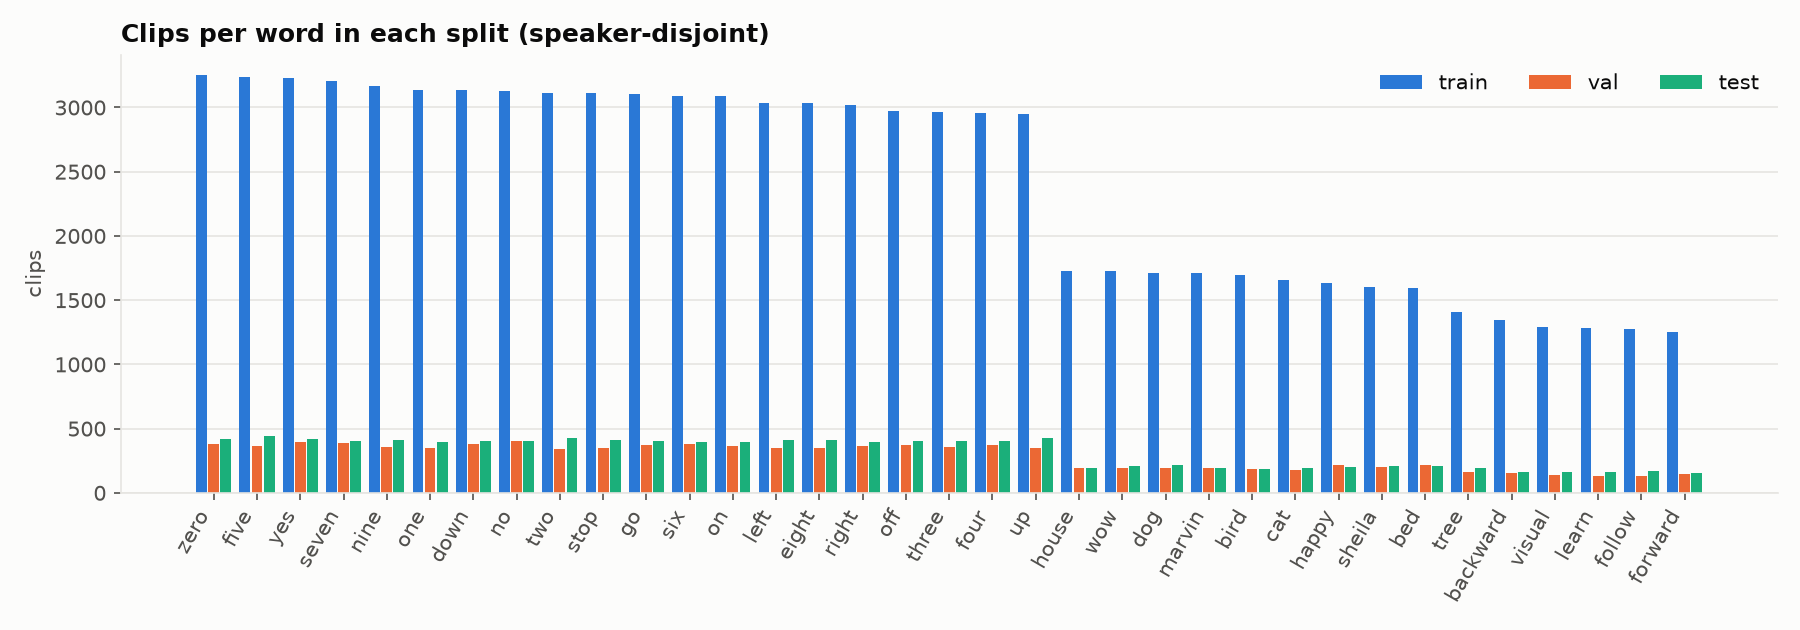
\includegraphics[width=\textwidth]{../outputs/report/01_dataset.png}
\caption{Número de clipes por palavra em cada partição. As $20$ palavras da esquerda são as principais do conjunto; as $15$ da direita têm cerca de metade dos exemplos.}
\label{fig:dataset}
\end{figure}

\subsection*{Controle de vazamento}

Com áudio de locutores reais, o vazamento mais comum é a mesma pessoa aparecer no treino e no teste: a rede aprende a voz e o microfone, e a acurácia de teste fica otimista. O carregamento dos dados (\texttt{speech\_data.check\_no\_leakage}) verifica que nenhum arquivo e nenhum locutor aparece em mais de uma partição. Além disso:
\begin{enumerate}
    \item a média e o desvio padrão usados para normalizar cada banda do log-mel foram calculados só sobre os clipes de treino;
    \item o aumento de dados é aplicado só aos lotes de treino, e validação e teste são avaliados com os clipes originais. As gravações de ruído não contêm fala, então não carregam rótulo nem identidade de locutor;
    \item a melhor época foi escolhida pela acurácia de validação, e o teste foi avaliado uma única vez, no fim;
    \item o script dos gráficos recarrega o \textit{checkpoint} salvo e confere que ele reproduz a acurácia de teste registrada no treino.
\end{enumerate}

\subsection*{O áudio como série temporal: espectrograma log-mel}

O problema é tratado como classificação de uma série temporal multivariada. Cada clipe é transformado numa sequência de $101$ vetores, um a cada $10\,\mathrm{ms}$, e cada vetor descreve como a energia do som está distribuída entre $40$ faixas de frequência naquele instante. A LSTM lê essa sequência passo a passo, do mesmo jeito que leria uma série de medições de um sensor, e só depois de percorrer os $101$ passos decide qual palavra foi dita. Essa sequência é o espectrograma log-mel, uma representação padrão em reconhecimento de fala.

Usar a forma de onda diretamente como série temporal seria possível, mas pouco prático, por três motivos:
\begin{enumerate}
    \item \textbf{Comprimento da sequência.} Um segundo a $16\,\mathrm{kHz}$ tem $16\,000$ amostras. Uma LSTM com $16\,000$ passos é lenta, porque os passos são processados em série, e tem dificuldade de propagar o gradiente por uma distância tão grande. Com o espectrograma a mesma informação cabe em $101$ passos.
    \item \textbf{O que identifica a palavra é o espectro, não a amostra.} Duas pessoas dizendo \w{yes} produzem formas de onda muito diferentes amostra a amostra, porque a fase e a altura da voz variam. O que se repete entre elas é a sequência de formantes (as faixas de frequência que o trato vocal reforça em cada vogal e consoante), que é exatamente o que o espectrograma mostra. Ao descartar a fase, o espectrograma remove uma fonte de variação que não ajuda a reconhecer a palavra.
    \item \textbf{Volume.} A amplitude da gravação depende da distância ao microfone e do ganho de cada aparelho, que no Speech Commands variam muito porque os clipes foram gravados por voluntários com equipamentos próprios~\cite{warden2018}.
\end{enumerate}

As duas operações que dão nome ao log-mel tratam dos dois últimos pontos. A escala mel agrupa as frequências do jeito que o ouvido humano as resolve: os filtros são estreitos nas frequências baixas, onde ficam os formantes que diferenciam as vogais, e largos nas altas, onde detalhes finos importam pouco para a fala. Isso reduz os $257$ coeficientes da FFT a $40$ bandas sem perder o que distingue as palavras; o uso de filtros na escala mel para reconhecimento de palavras vem de Davis e Mermelstein~\cite{davis1980}. O logaritmo comprime a faixa dinâmica, de forma parecida com a percepção de volume, e transforma um ganho multiplicativo do microfone num deslocamento aditivo, que a normalização por banda remove em boa parte.

O cálculo (\texttt{src/speech\_data.py}) segue os passos usuais. Clipes com menos de $16\,000$ amostras recebem zeros no final. O sinal é cortado em janelas de Hann de $25\,\mathrm{ms}$ ($400$ amostras) com passo de $10\,\mathrm{ms}$ ($160$ amostras), o que dá $101$ quadros. Cada quadro passa por uma FFT de $512$ pontos ($257$ coeficientes entre $0$ e $8\,\mathrm{kHz}$), o espectro de potência é somado por $40$ filtros triangulares na escala mel entre $20\,\mathrm{Hz}$ e $8\,\mathrm{kHz}$, e aplica-se o logaritmo:
\begin{equation}
    X_{t,m} = \log\!\Big(\sum_{k} H_m(k)\,\big|\mathrm{FFT}(w \cdot x_t)(k)\big|^2 + 10^{-6}\Big), \qquad t = 1,\dots,101, \quad m = 1,\dots,40,
\end{equation}
em que $x_t$ é o quadro $t$, $w$ a janela de Hann e $H_m$ o $m$-ésimo filtro mel. Cada banda $m$ é então normalizada com a média e o desvio padrão do treino. A entrada da rede é a série $\mathbf{X} = (\mathbf{x}_1, \dots, \mathbf{x}_{101})$, com $\mathbf{x}_t \in \mathbb{R}^{40}$. O cálculo é feito na GPU a cada lote, e o banco de filtros mel foi implementado em numpy.

A Figura~\ref{fig:audio} mostra quatro exemplos. No espectrograma, o eixo horizontal é o tempo da série e cada coluna é um vetor $\mathbf{x}_t$. A palavra ocupa uma parte do segundo, e a posição varia: em \w{yes} ela começa perto de $0{,}65\,\mathrm{s}$, em \w{three} logo no início. O par \w{tree}/\w{three} já mostra a dificuldade que aparece adiante. As duas palavras diferem quase só na consoante inicial, que dura poucos quadros.

\begin{figure}[H]
\centering
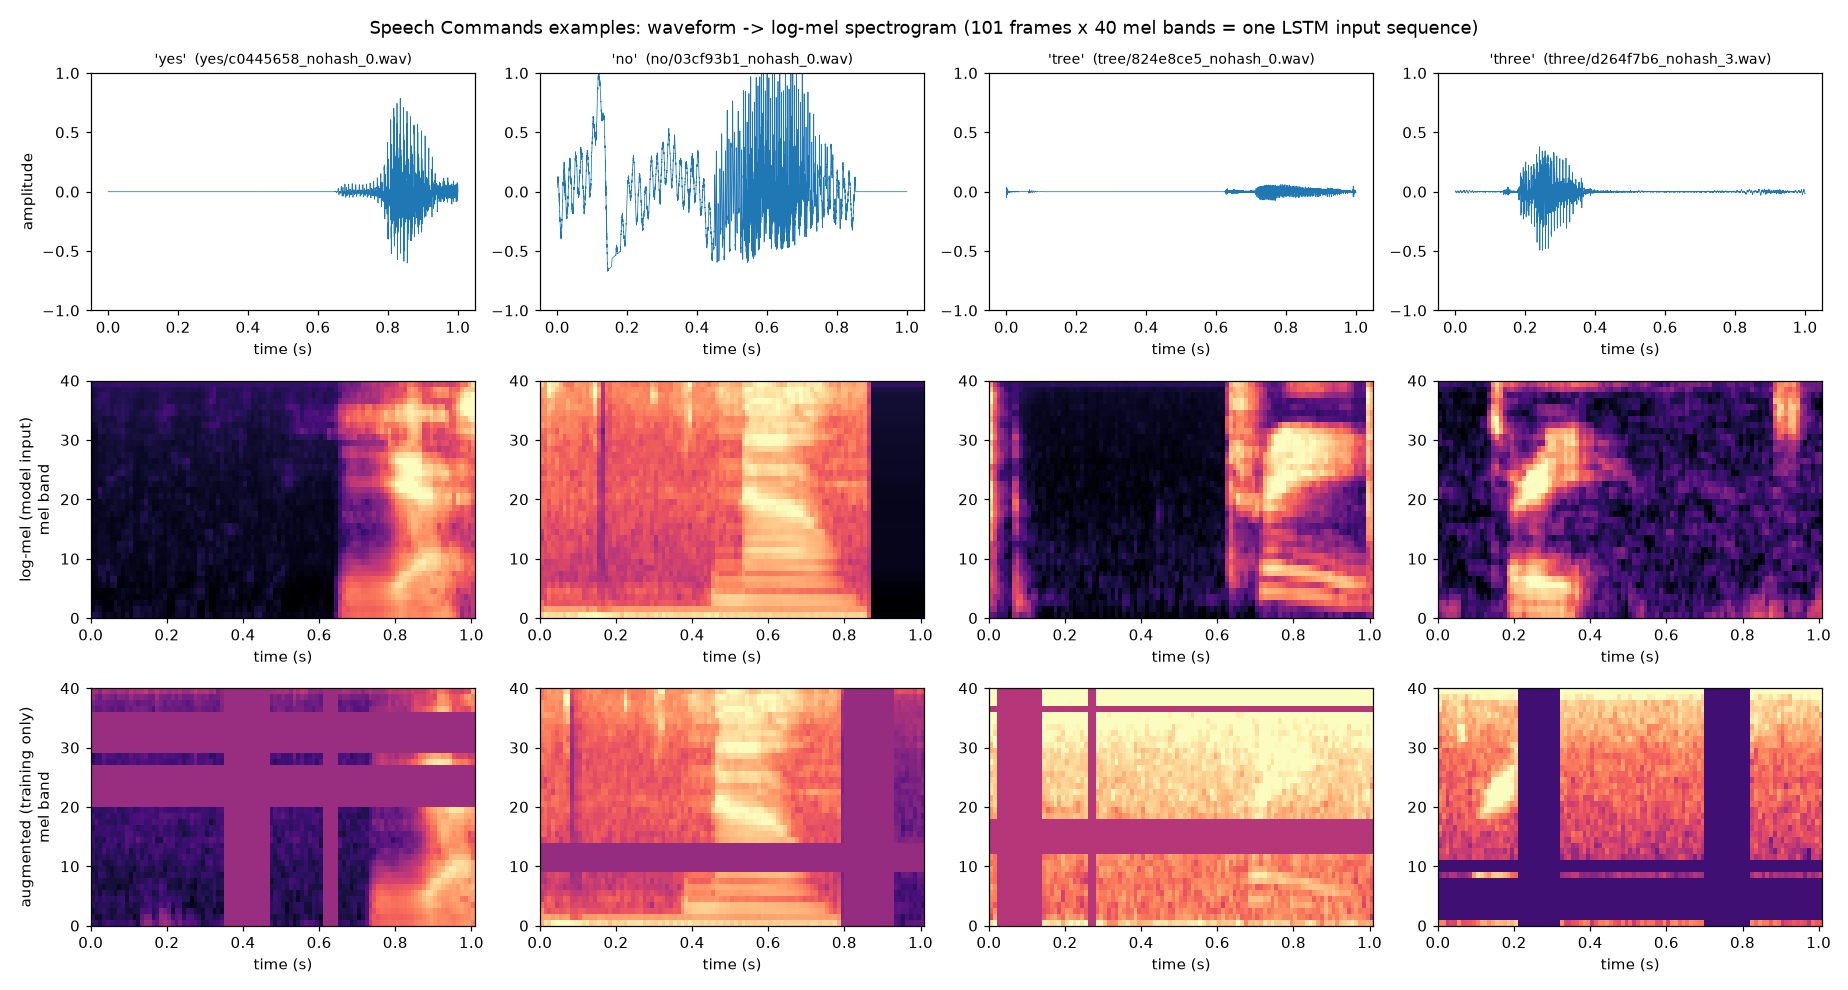
\includegraphics[width=\textwidth]{../outputs/audio_examples.png}
\caption{Quatro clipes do conjunto. Primeira linha: forma de onda. Segunda: espectrograma log-mel normalizado, que é a entrada da rede. Terceira: o mesmo espectrograma depois do aumento de dados usado no treino (deslocamento, ruído de fundo e máscaras do SpecAugment).}
\label{fig:audio}
\end{figure}

\subsection*{Modelo}

O classificador (\texttt{src/model.py}) é uma LSTM~\cite{hochreiter1997} bidirecional de duas camadas (Figura~\ref{fig:model}). A LSTM é uma rede recorrente: a cada passo $t$ ela combina o quadro $\mathbf{x}_t$ com o estado que carregou do passo anterior, $\mathbf{h}_t = \mathrm{LSTM}(\mathbf{x}_t, \mathbf{h}_{t-1})$, e as portas internas decidem o que guardar e o que esquecer. Assim o estado em cada instante resume o trecho da série já lido, por exemplo que uma consoante fricativa acabou de ser ouvida e uma vogal está começando. Primeiro uma \textit{LayerNorm} normaliza os $40$ valores de cada quadro. Em cada camada, uma LSTM lê a sequência do início para o fim e outra do fim para o início, cada uma com $256$ unidades, e as saídas das duas são concatenadas em $512$ valores por quadro. Entre as camadas há \textit{dropout} de $0{,}2$. Ler a sequência nos dois sentidos é válido aqui porque o clipe inteiro está disponível quando a classificação é feita; não existe ``futuro'' que a rede pudesse espiar.

Para resumir a sequência num único vetor, as saídas da segunda camada passam por média e máximo ao longo do tempo, que concatenados dão $1\,024$ valores. A alternativa comum, usar só a saída do último passo, deixaria a direção reversa com apenas um quadro de contexto, já que no último instante ela acabou de começar a leitura. Com a média e o máximo todos os quadros contribuem, e o máximo deixa a rede responder a um trecho curto e característico em qualquer posição do clipe. A cabeça de classificação é \textit{Dropout} $\to$ Linear($1024 \to 512$) $\to$ GELU $\to$ \textit{Dropout} $\to$ Linear($512 \to 35$). O modelo tem $2{,}73$ milhões de parâmetros, dos quais $2{,}19$ milhões estão nas LSTMs.

\begin{figure}[H]
\centering
\begin{tikzpicture}[node distance=0.45cm and 0.42cm]
    \node[layer=gray!15] (x) {log-mel\\[-1pt]\scriptsize $101{\times}40$};
    \node[layer=gray!8, right=of x] (ln) {\scriptsize Layer\\[-2pt]\scriptsize Norm};
    \node[layer, right=0.75cm of ln, yshift=0.65cm] (f1) {\scriptsize LSTM $\rightarrow$\\[-2pt]\scriptsize 256};
    \node[layer, below=0.3cm of f1] (b1) {\scriptsize LSTM $\leftarrow$\\[-2pt]\scriptsize 256};
    \node[layer, right=0.75cm of f1] (f2) {\scriptsize LSTM $\rightarrow$\\[-2pt]\scriptsize 256};
    \node[layer, below=0.3cm of f2] (b2) {\scriptsize LSTM $\leftarrow$\\[-2pt]\scriptsize 256};
    \node[layer=orange!15, right=0.75cm of f2] (mean) {\scriptsize média\\[-2pt]\scriptsize 512};
    \node[layer=orange!15, right=0.75cm of b2] (max) {\scriptsize máximo\\[-2pt]\scriptsize 512};
    \node[layer=green!12] (cat) at ($(mean)!0.5!(max) + (1.7,0)$) {\scriptsize concat\\[-2pt]\scriptsize 1024};
    \node[layer=red!8, right=of cat] (h1) {\scriptsize Linear\\[-2pt]\scriptsize 512, GELU};
    \node[layer=red!8, right=of h1] (h2) {\scriptsize Linear\\[-2pt]\scriptsize 35};
    \node[layer=gray!15, right=of h2] (y) {logits\\[-1pt]\scriptsize 35};

    \draw[arrow] (x) -- (ln);
    \draw[arrow] (ln.east) -- (f1.west);
    \draw[arrow] (ln.east) -- (b1.west);
    \draw[arrow] (f1) -- (f2);
    \draw[arrow] (b1) -- (b2);
    \draw[arrow] (f1.east) -- (b2.west);
    \draw[arrow] (b1.east) -- (f2.west);
    \draw[arrow] (f2.east) -- (mean.west);
    \draw[arrow] (b2.east) -- (mean.west);
    \draw[arrow] (f2.east) -- (max.west);
    \draw[arrow] (b2.east) -- (max.west);
    \draw[arrow] (mean.east) -- (cat.west);
    \draw[arrow] (max.east) -- (cat.west);
    \draw[arrow] (cat) -- (h1);
    \draw[arrow] (h1) -- (h2);
    \draw[arrow] (h2) -- (y);

    \begin{scope}[on background layer]
        \node[draw=blue!50, dashed, rounded corners, fit=(f1)(b1), inner sep=4pt,
              label={[lbl, blue!60!black]above:camada 1}] {};
        \node[draw=blue!50, dashed, rounded corners, fit=(f2)(b2), inner sep=4pt,
              label={[lbl, blue!60!black]above:camada 2}] {};
        \node[draw=orange!60, dashed, rounded corners, fit=(mean)(max), inner sep=4pt,
              label={[lbl, orange!60!black]above:pooling no tempo}] {};
        \node[draw=red!50, dashed, rounded corners, fit=(h1)(h2), inner sep=4pt,
              label={[lbl, red!60!black]above:cabeça MLP}] {};
    \end{scope}
\end{tikzpicture}
\caption{Arquitetura do classificador. Cada camada recorrente tem uma LSTM em cada sentido, com saídas concatenadas ($512$ valores por quadro); a segunda camada recebe a saída concatenada da primeira. Os números indicam a largura de cada bloco. Há \textit{dropout} de $0{,}2$ entre as camadas LSTM e antes de cada camada linear.}
\label{fig:model}
\end{figure}

O modelo devolve \textit{logits}, sem softmax na saída. A função de perda \texttt{CrossEntropyLoss} aplica o log-softmax internamente, que é numericamente mais estável do que calcular o softmax e depois o logaritmo. As probabilidades são obtidas com $\mathrm{softmax}(\text{logits})$ na inferência. A softmax é a escolha certa porque as classes são mutuamente exclusivas: cada clipe tem uma única palavra, e as probabilidades devem somar $1$. Sigmoides independentes serviriam para um problema com vários rótulos por exemplo, que não é o caso.

\subsection*{Treinamento}

O otimizador foi o AdamW com decaimento de pesos $10^{-2}$ e taxa de aprendizado no esquema \textit{one-cycle}, que sobe até $2 \times 10^{-3}$ e depois desce até perto de zero ao longo das $40$ épocas. Os lotes têm $256$ clipes, a norma do gradiente é limitada a $1{,}0$ e a semente é $0$. A perda é a entropia cruzada com suavização de rótulos de $0{,}1$: o alvo deixa de ser $1$ para a classe certa e $0$ para as outras e passa a ser
\begin{equation}
    \tilde{y}_k = (1 - \varepsilon)\,\mathbb{1}[k = y] + \frac{\varepsilon}{35}, \qquad \varepsilon = 0{,}1,
\end{equation}
ou seja, cerca de $0{,}903$ para a classe certa e $0{,}003$ para cada uma das outras. Isso desestimula a rede de empurrar as probabilidades para os extremos. O conjunto de treino inteiro fica na GPU como formas de onda em \texttt{int16}, e os espectrogramas e o aumento de dados são calculados a cada lote, então cada época vê versões aumentadas diferentes dos clipes.

O aumento de dados, aplicado só ao treino, tem três etapas nesta ordem:
\begin{enumerate}
    \item \textbf{Deslocamento no tempo:} o clipe é deslocado aleatoriamente em até $\pm 100\,\mathrm{ms}$, com zeros preenchendo o espaço que sobra. Isso ensina que a palavra pode aparecer em qualquer ponto do segundo.
    \item \textbf{Ruído de fundo:} em $80\%$ dos clipes soma-se um trecho aleatório de $1$ segundo das gravações de ruído, com ganho sorteado uniformemente entre $0$ e $0{,}1$ da escala cheia.
    \item \textbf{SpecAugment}~\cite{park2019}\textbf{:} sobre o log-mel já normalizado, duas faixas de frequência (até $8$ bandas cada) e duas faixas de tempo (até $12$ quadros cada) são zeradas. Como o espectrograma está normalizado, zero corresponde à média do treino. A rede precisa então reconhecer a palavra mesmo com partes do espectro faltando.
\end{enumerate}
A terceira linha da Figura~\ref{fig:audio} mostra o efeito combinado. Em \w{tree}, o ruído somado é mais forte que a própria fala e quase apaga a palavra.

\section{Resultados de Treinamento}

A Figura~\ref{fig:curves} mostra as curvas e a Tabela~\ref{tab:curve} alguns pontos delas. A acurácia de validação passa de $90\%$ na época $10$ e cresce devagar depois disso, chegando ao máximo de $95{,}96\%$ na época $36$, cujos pesos foram mantidos. Nas últimas quatro épocas ela fica estável em torno de $95{,}9\%$, sem queda que indique sobreajuste.

\begin{figure}[H]
\centering
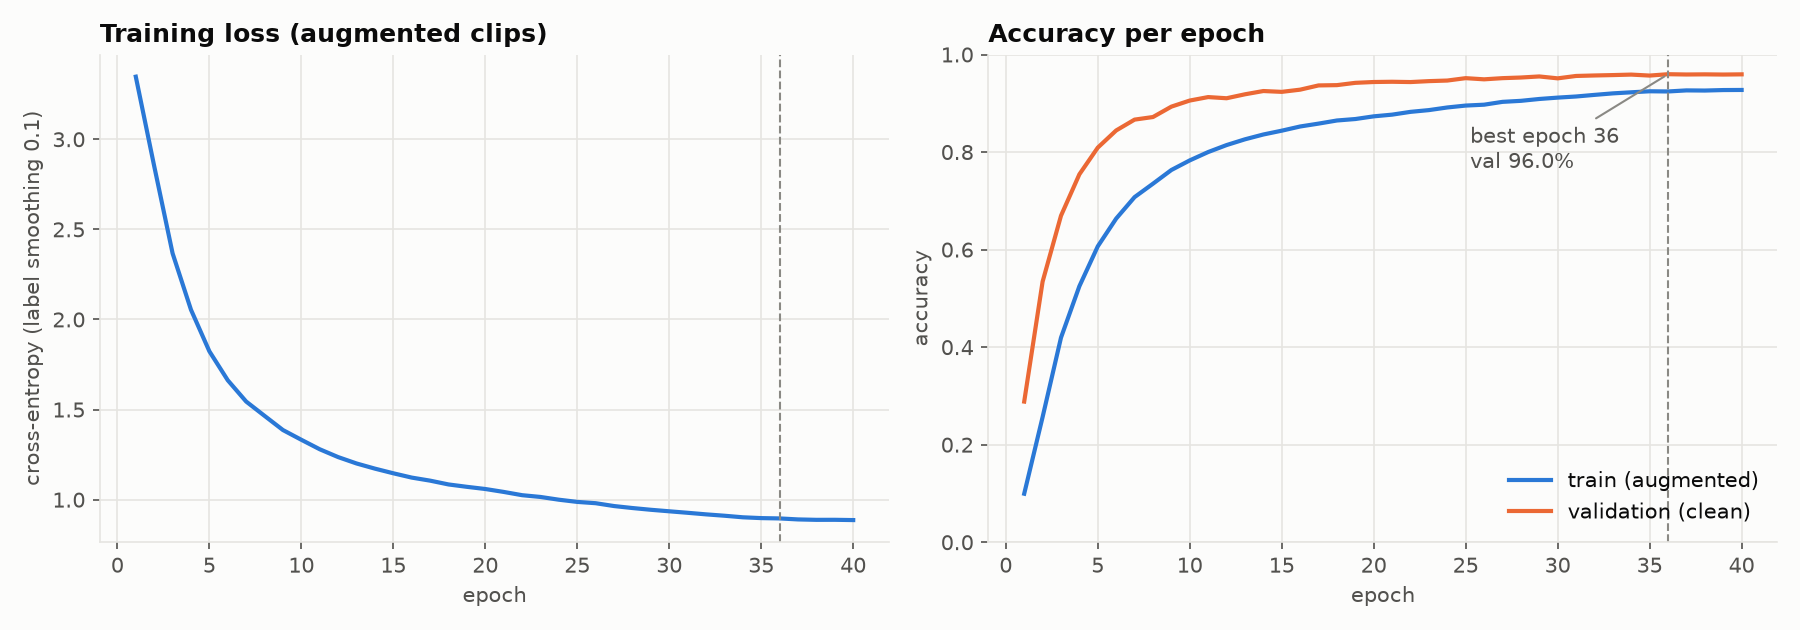
\includegraphics[width=\textwidth]{../outputs/report/02_training_curves.png}
\caption{Perda de treino (com suavização de rótulos, sobre clipes aumentados) e acurácia de treino e validação por época. A linha tracejada marca a época $36$, escolhida pela validação.}
\label{fig:curves}
\end{figure}

\begin{table}[H]
\centering
\caption{Perda e acurácia em algumas épocas. A perda de treino é medida nos clipes aumentados e inclui a suavização de rótulos.}
\label{tab:curve}
\small
\begin{tabular}{rrrr}
\toprule
Época & Perda de treino & Acurácia de treino & Acurácia de validação \\
\midrule
1  & 3,347 & 9,9\%  & 28,8\% \\
10 & 1,332 & 78,3\% & 90,6\% \\
20 & 1,059 & 87,3\% & 94,4\% \\
30 & 0,936 & 91,2\% & 95,1\% \\
36 (melhor) & 0,896 & 92,4\% & 96,0\% \\
40 & 0,887 & 92,7\% & 95,9\% \\
\bottomrule
\end{tabular}
\end{table}

A acurácia de validação fica acima da de treino durante todo o treino, o contrário do que se costuma ver. A diferença vem do aumento de dados: os clipes de treino recebem ruído, deslocamento e máscaras, e por isso são mais difíceis que os de validação, que são limpos. O \textit{dropout}, ativo só no treino, contribui no mesmo sentido. A perda de treino não chega perto de zero porque a suavização de rótulos impõe um piso. Mesmo um modelo que acertasse o alvo $\tilde{y}$ perfeitamente teria entropia cruzada de cerca de $0{,}66$.

\section{Desempenho no Teste}

Avaliado uma única vez sobre os $11\,005$ clipes de teste, de $250$ locutores que a rede nunca ouviu, o modelo acertou $10\,465$, uma acurácia de $95{,}09\%$. Um palpite aleatório acertaria $1/35 = 2{,}86\%$. A diferença de menos de um ponto em relação à validação ($95{,}96\%$) é compatível com a troca de locutores entre as duas partições. A Tabela~\ref{tab:final} resume as métricas.

\begin{table}[H]
\centering
\caption{Métricas finais do modelo da época $36$.}
\label{tab:final}
\small
\begin{tabular}{lr}
\toprule
Métrica & Valor \\
\midrule
Acurácia de teste & 95,09\% (10\,465 / 11\,005) \\
Acurácia de validação (época 36) & 95,96\% \\
Acurácia de um palpite aleatório & 2,86\% \\
F1 macro (teste) & 0,948 \\
Erro de calibração esperado (ECE, 15 faixas) & 0,085 \\
\bottomrule
\end{tabular}
\end{table}

O F1 macro, média simples do F1 das $35$ classes, é $0{,}948$, muito perto da acurácia. As palavras auxiliares, com metade dos exemplos de treino, não ficam sistematicamente para trás. A Figura~\ref{fig:perclass} mostra precisão, revocação e F1 por palavra. As mais fáceis são \w{stop} ($0{,}982$), \w{yes} ($0{,}976$), \w{seven} e \w{zero} ($0{,}973$) e \w{marvin} ($0{,}969$). As mais difíceis são \w{tree} ($0{,}862$), \w{learn} ($0{,}894$), \w{forward} ($0{,}902$), \w{up} ($0{,}923$), \w{follow} ($0{,}925$) e \w{bed} ($0{,}931$). Das seis piores, quatro estão entre as menos representadas no treino, mas o que elas têm em comum, como mostra a seção seguinte, é ter uma palavra parecida na lista.

\begin{figure}[H]
\centering
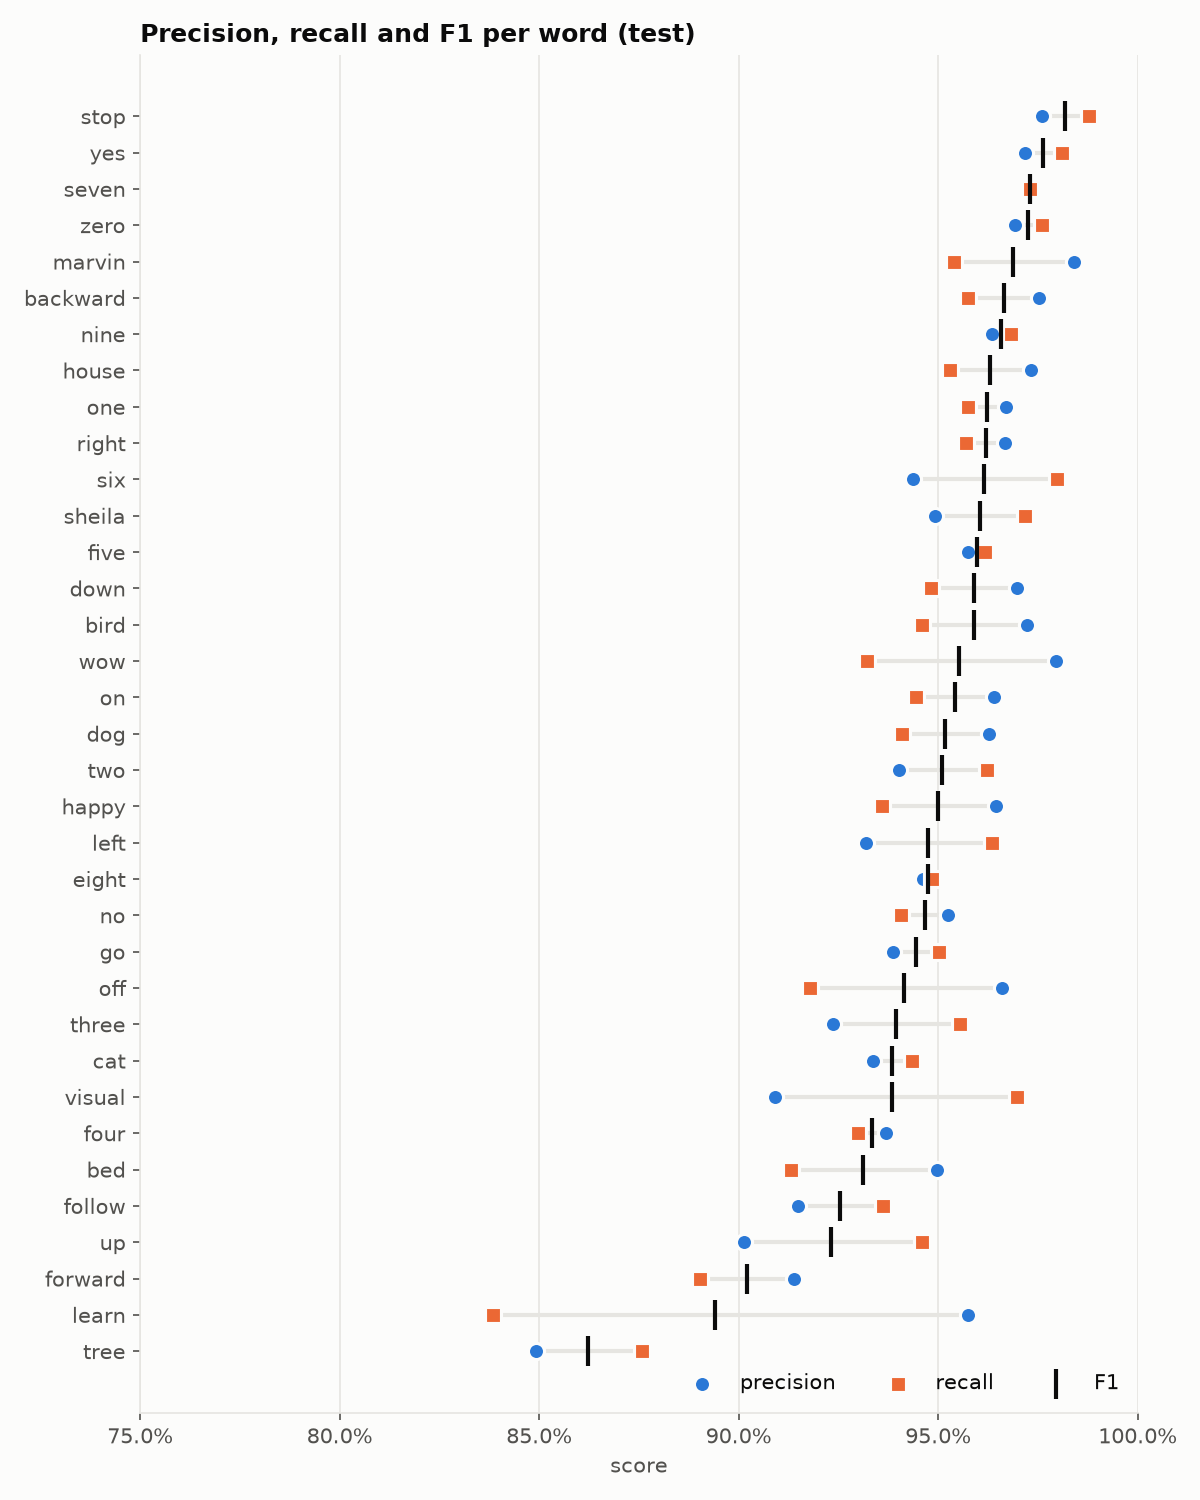
\includegraphics[width=\textwidth]{../outputs/report/05_per_class_metrics.png}
\caption{Precisão, revocação e F1 de cada palavra no conjunto de teste.}
\label{fig:perclass}
\end{figure}

\w{learn} é o caso em que precisão e revocação mais se afastam: precisão de $0{,}957$ e revocação de $0{,}839$. Quando o modelo diz \w{learn} ele quase sempre acerta, mas $16\%$ dos \w{learn} verdadeiros recebem outro rótulo, e o destino mais comum é \w{left}. \w{tree} é ruim nos dois sentidos (precisão $0{,}849$, revocação $0{,}876$), porque erra para \w{three} e também recebe exemplos de \w{three}.

\section{Análise dos Erros}

A Figura~\ref{fig:confusion} traz a matriz de confusão normalizada por linha, e a Figura~\ref{fig:topconf} os $15$ erros mais frequentes. A diagonal concentra quase toda a massa, e os poucos valores fora dela que chegam a $2\%$ aparecem em grupos pequenos de palavras. Os erros mais comuns (palavra verdadeira $\to$ prevista) são \w{off}$\to$\w{up} ($17$ clipes), \w{tree}$\to$\w{three} ($15$), \w{learn}$\to$\w{left} ($11$), \w{four}$\to$\w{forward} ($11$), \w{forward}$\to$\w{four} ($10$), \w{three}$\to$\w{tree} ($10$) e \w{four}$\to$\w{follow} ($8$), seguidos de \w{two}$\to$\w{zero}, \w{up}$\to$\w{off}, \w{up}$\to$\w{on} e \w{on}$\to$\w{up}, com $6$ cada.

\begin{figure}[H]
\centering
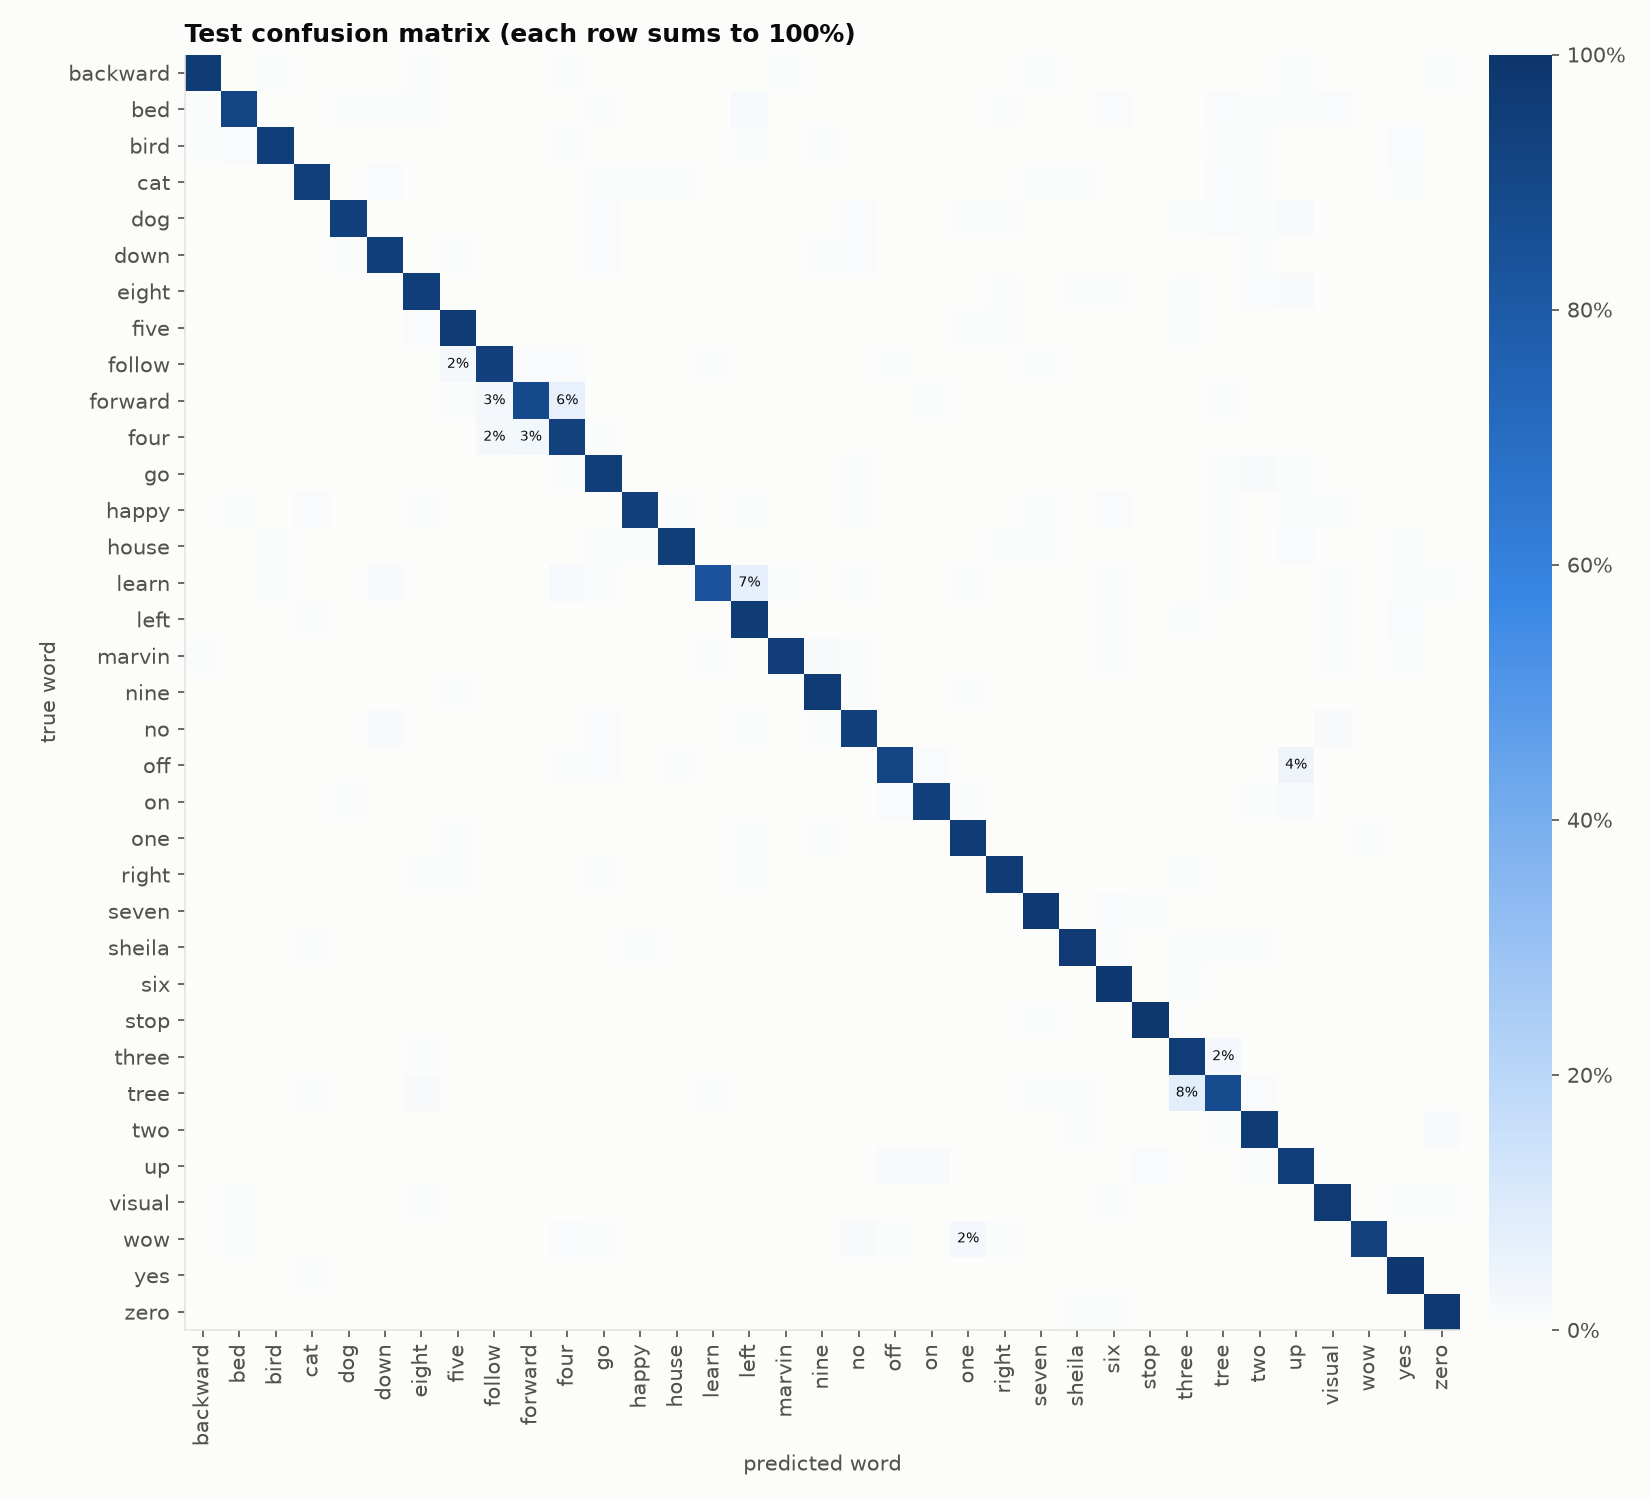
\includegraphics[width=0.88\textwidth]{../outputs/report/03_confusion_matrix.png}
\caption{Matriz de confusão do teste, normalizada por linha (cada linha soma $100\%$). Os valores fora da diagonal a partir de $2\%$ estão anotados.}
\label{fig:confusion}
\end{figure}

\begin{figure}[H]
\centering
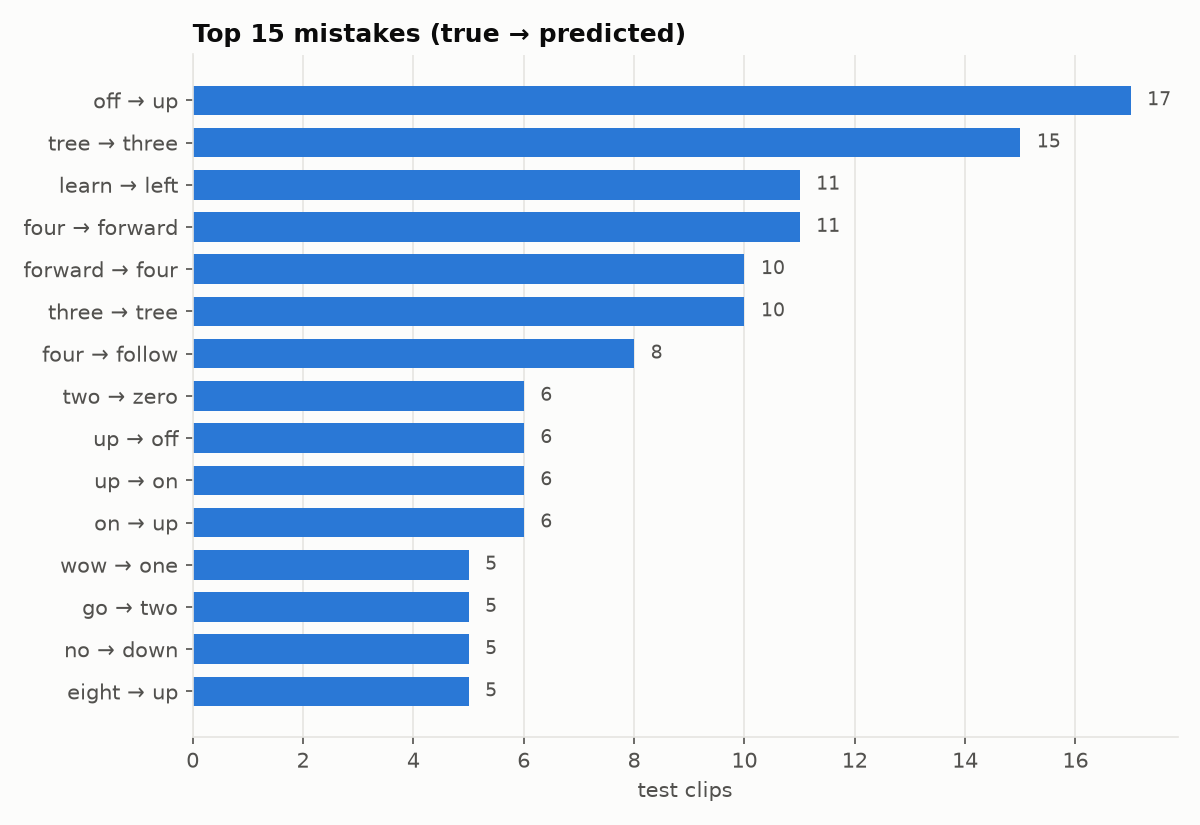
\includegraphics[width=0.8\textwidth]{../outputs/report/04_top_confusions.png}
\caption{Os $15$ pares (palavra verdadeira $\to$ palavra prevista) mais frequentes entre os erros do teste.}
\label{fig:topconf}
\end{figure}

Quase todos esses pares são acusticamente próximos, e a semelhança ajuda a explicar cada um. \w{tree} e \w{three} diferem só no começo, \textit{tr} contra \textit{thr}, e o \textit{th} é um som fraco, de pouca energia, que some com facilidade num microfone ruim ou com ruído de fundo; $8\%$ dos \w{tree} viram \w{three}. \w{four}, \w{forward} e \w{follow} começam todos com /f/ seguido de vogal posterior, e \w{forward} é praticamente \w{four} com uma segunda sílaba fraca no fim. \w{learn} e \w{left} começam igual, com /l/ e vogal média. \w{off}, \w{up} e \w{on} são monossílabos curtos, com vogal parecida e consoante final de pouca energia. Os erros, portanto, não se espalham ao acaso entre as $35$ classes: eles se concentram em pares mínimos e quase pares mínimos, onde a informação que distingue as palavras está em poucos quadros do espectrograma. Essa é também a parte do sinal que o SpecAugment às vezes apaga no treino e que o ruído encobre primeiro.

\subsection{Erros com alta confiança e ruído nos rótulos}

A Figura~\ref{fig:mistakes} mostra os $12$ erros em que o modelo estava mais confiante. Alguns são confusões plausíveis, como \w{three}$\to$\w{tree} com $94\%$ e $92\%$ de confiança, e \w{learn}$\to$\w{left} com $93\%$. Outros são difíceis de explicar pelo som e parecem ser problemas do próprio rótulo. No clipe de \w{sheila} classificado como \w{two} ($97\%$), o espectrograma mostra uma faixa de ruído constante e só uma mancha curta de energia nas bandas baixas, sem a estrutura de duas sílabas que \w{sheila} teria. No clipe de \w{six} classificado como \w{sheila} ($92\%$), a gravação é cortada pouco depois de $0{,}55\,\mathrm{s}$, e o que sobra é um som sibilante longo, que de fato lembra o início de \w{sheila}. O Speech Commands foi coletado com voluntários pela internet, e esse tipo de ruído de rótulo é uma característica conhecida do conjunto. A inspeção aqui é visual e não confirma qual era a palavra gravada, mas sugere que parte dos $4{,}9\%$ de erro não está ao alcance de nenhum classificador.

\begin{figure}[H]
\centering
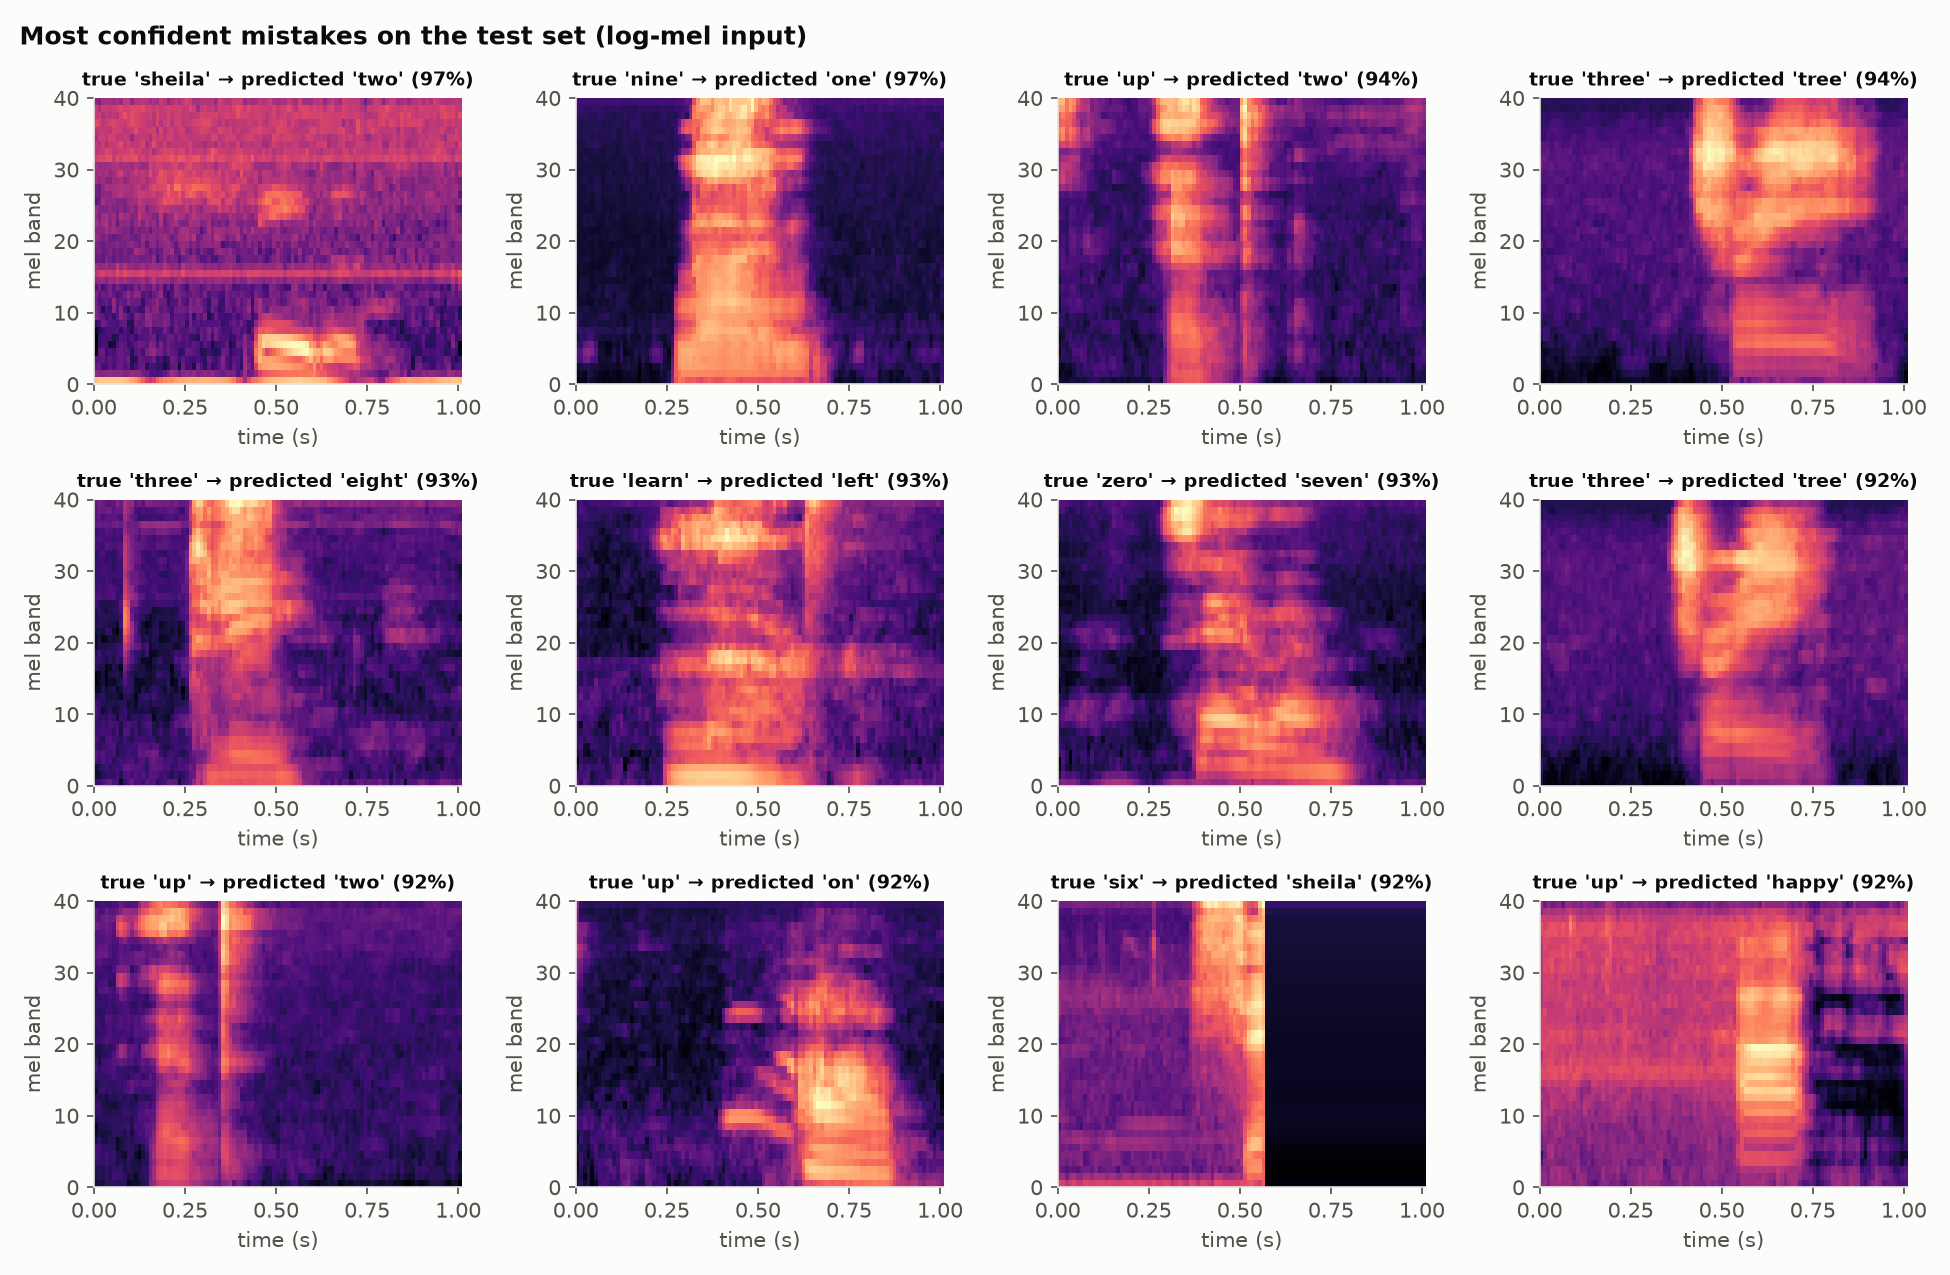
\includegraphics[width=\textwidth]{../outputs/report/09_misclassified.png}
\caption{Espectrogramas log-mel dos $12$ erros de teste com maior confiança, com a palavra verdadeira, a prevista e a probabilidade atribuída à classe prevista.}
\label{fig:mistakes}
\end{figure}

\section{Robustez ao Ruído}

Para medir o quanto o modelo tolera ruído, os clipes de teste foram reavaliados com ruído de fundo somado a uma relação sinal-ruído (SNR) fixa:
\begin{equation}
    \mathrm{SNR} = 10 \log_{10} \frac{P_{\text{fala}}}{P_{\text{ruído}}}\ \mathrm{dB},
\end{equation}
em que $P_{\text{fala}}$ é a potência média do trecho de $0{,}25\,\mathrm{s}$ mais forte do clipe, para que o silêncio antes e depois da palavra não reduza a estimativa. Em $0\,\mathrm{dB}$ o ruído tem a mesma potência da fala. A Tabela~\ref{tab:snr} e a Figura~\ref{fig:snr} trazem os resultados.

\begin{table}[H]
\centering
\caption{Acurácia de teste com ruído de fundo somado a uma SNR fixa.}
\label{tab:snr}
\small
\begin{tabular}{lrrrrrr}
\toprule
SNR & sem ruído & 20 dB & 10 dB & 5 dB & 0 dB & $-5$ dB \\
\midrule
Acurácia & 95,1\% & 93,7\% & 87,0\% & 77,6\% & 61,1\% & 36,5\% \\
\bottomrule
\end{tabular}
\end{table}

\begin{figure}[H]
\centering
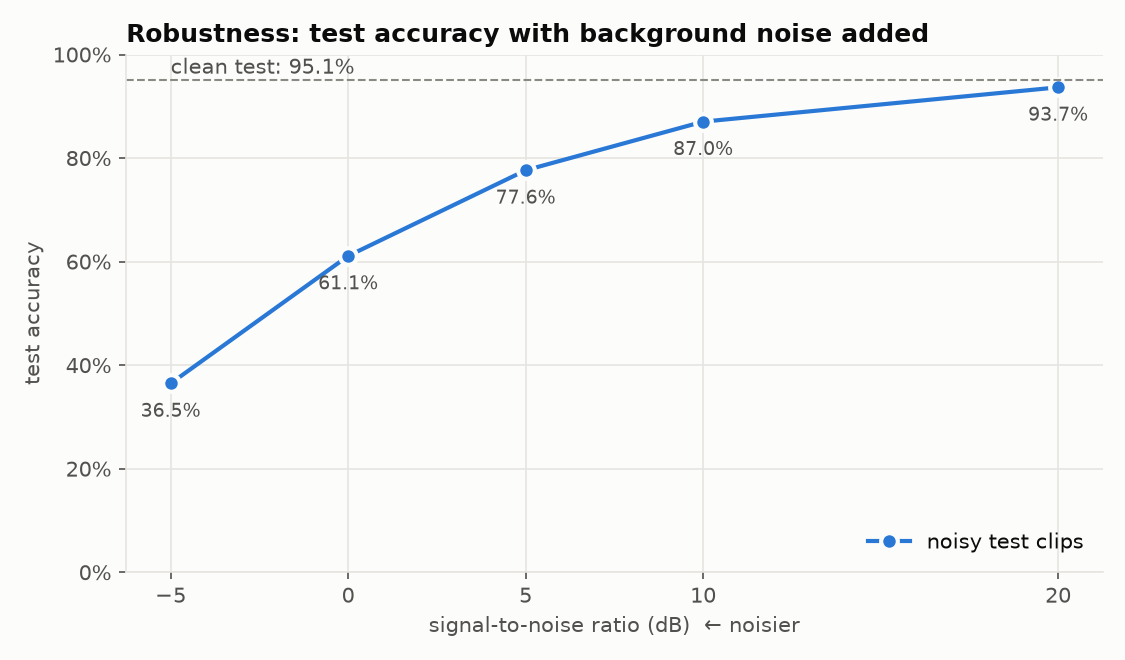
\includegraphics[width=0.7\textwidth]{../outputs/report/07_noise_robustness.png}
\caption{Acurácia de teste em função da SNR do ruído somado aos clipes.}
\label{fig:snr}
\end{figure}

A $20\,\mathrm{dB}$ a perda é de $1{,}4$ ponto. A partir de $10\,\mathrm{dB}$ a queda acelera, e a $0\,\mathrm{dB}$ o modelo ainda acerta $61\%$, mais de vinte vezes o acaso. Há uma ressalva importante: o ruído do teste vem das mesmas seis gravações usadas no aumento de dados do treino, ainda que em trechos sorteados de novo. Esses números medem a robustez a tipos de ruído que a rede já conhece, e um ruído de natureza diferente (vozes ao fundo, música, reverberação) provavelmente causaria uma queda maior. Um teste mais justo exigiria gravações de ruído separadas para o treino e para a avaliação.

\section{Calibração}

Uma rede bem calibrada acerta cerca de $80\%$ das vezes em que diz ter $80\%$ de confiança. Para medir isso, os clipes de teste foram divididos em $15$ faixas de confiança (a maior probabilidade da softmax), e o erro de calibração esperado (ECE) é a média ponderada da diferença entre acurácia e confiança em cada faixa:
\begin{equation}
    \mathrm{ECE} = \sum_{b=1}^{15} \frac{n_b}{N} \,\big|\mathrm{acc}(b) - \mathrm{conf}(b)\big|.
\end{equation}

\begin{figure}[H]
\centering
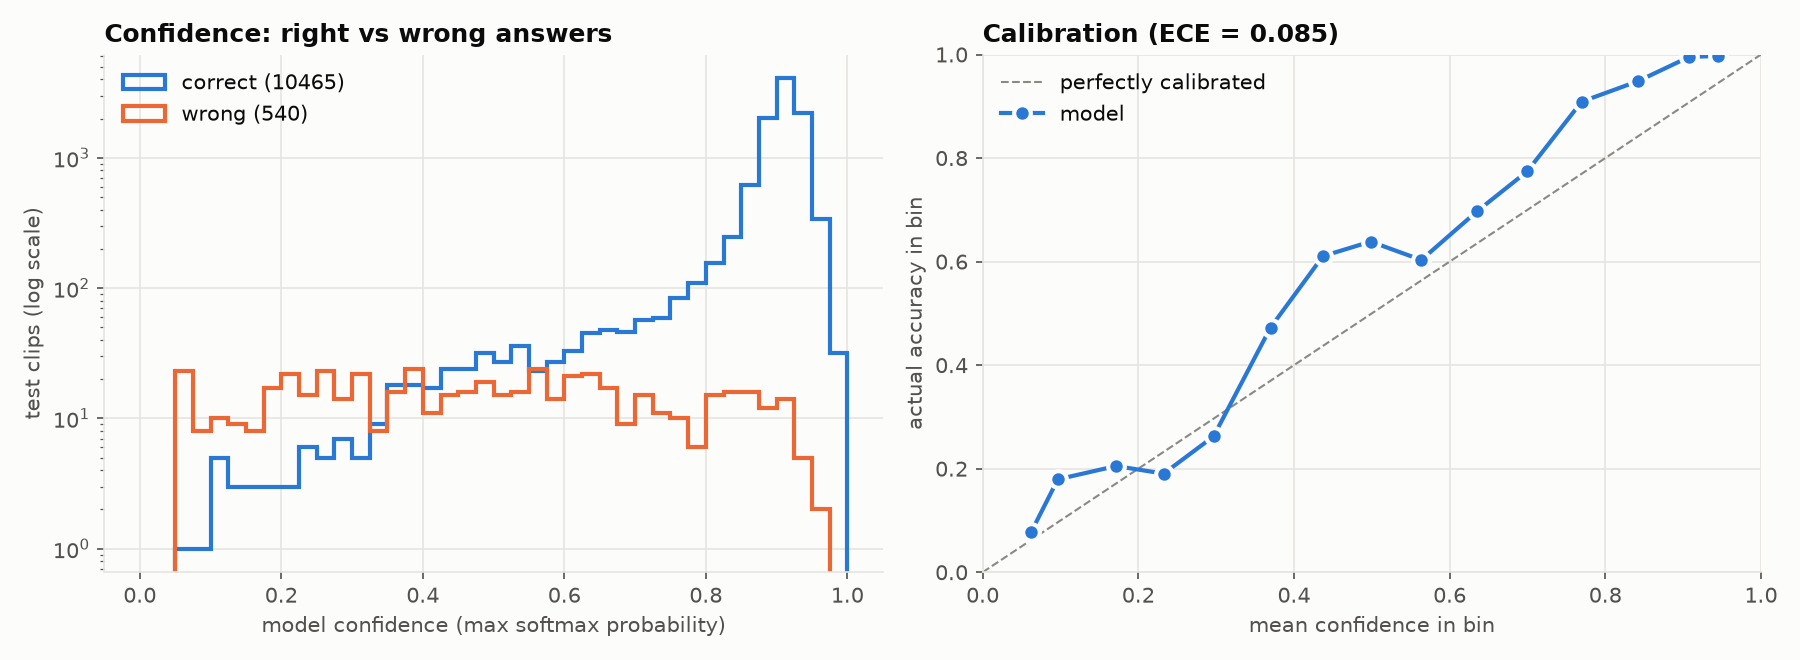
\includegraphics[width=\textwidth]{../outputs/report/06_confidence.png}
\caption{Esquerda: histograma da confiança nos acertos e nos erros do teste (eixo vertical em escala logarítmica). Direita: diagrama de confiabilidade; a diagonal tracejada corresponde a uma calibração perfeita.}
\label{fig:conf}
\end{figure}

O ECE é $0{,}085$, e a Figura~\ref{fig:conf} mostra a direção do desvio. A partir de uma confiança de cerca de $0{,}35$, os pontos do diagrama ficam acima da diagonal: na faixa em que o modelo diz ter $0{,}84$ de confiança, por exemplo, ele acerta $95\%$. O modelo é subconfiante, efeito esperado da suavização de rótulos, que treina a rede para nunca passar de cerca de $0{,}90$ na classe certa. O histograma confirma isso. Quase todos os acertos têm confiança entre $0{,}85$ e $0{,}95$, e muito poucos passam de $0{,}97$. Os $540$ erros se espalham de forma quase uniforme entre $0{,}05$ e $0{,}95$. A confiança separa bem os dois grupos, então ela serve para filtrar respostas duvidosas, mas o valor numérico não deve ser lido como uma probabilidade exata. Se isso fosse necessário, um ajuste de temperatura sobre a validação corrigiria a escala sem alterar as previsões.

\section{O que a Rede Aprendeu}

Para ver como a rede organiza as palavras, foi extraída a ativação de $512$ dimensões da camada oculta da cabeça (depois da GELU) para $80$ clipes de teste de cada palavra, e esses vetores foram projetados em 2D com o t-SNE (perplexidade $30$, inicialização pela PCA). O t-SNE procura uma disposição no plano em que pontos vizinhos no espaço original continuem vizinhos.

\begin{figure}[H]
\centering
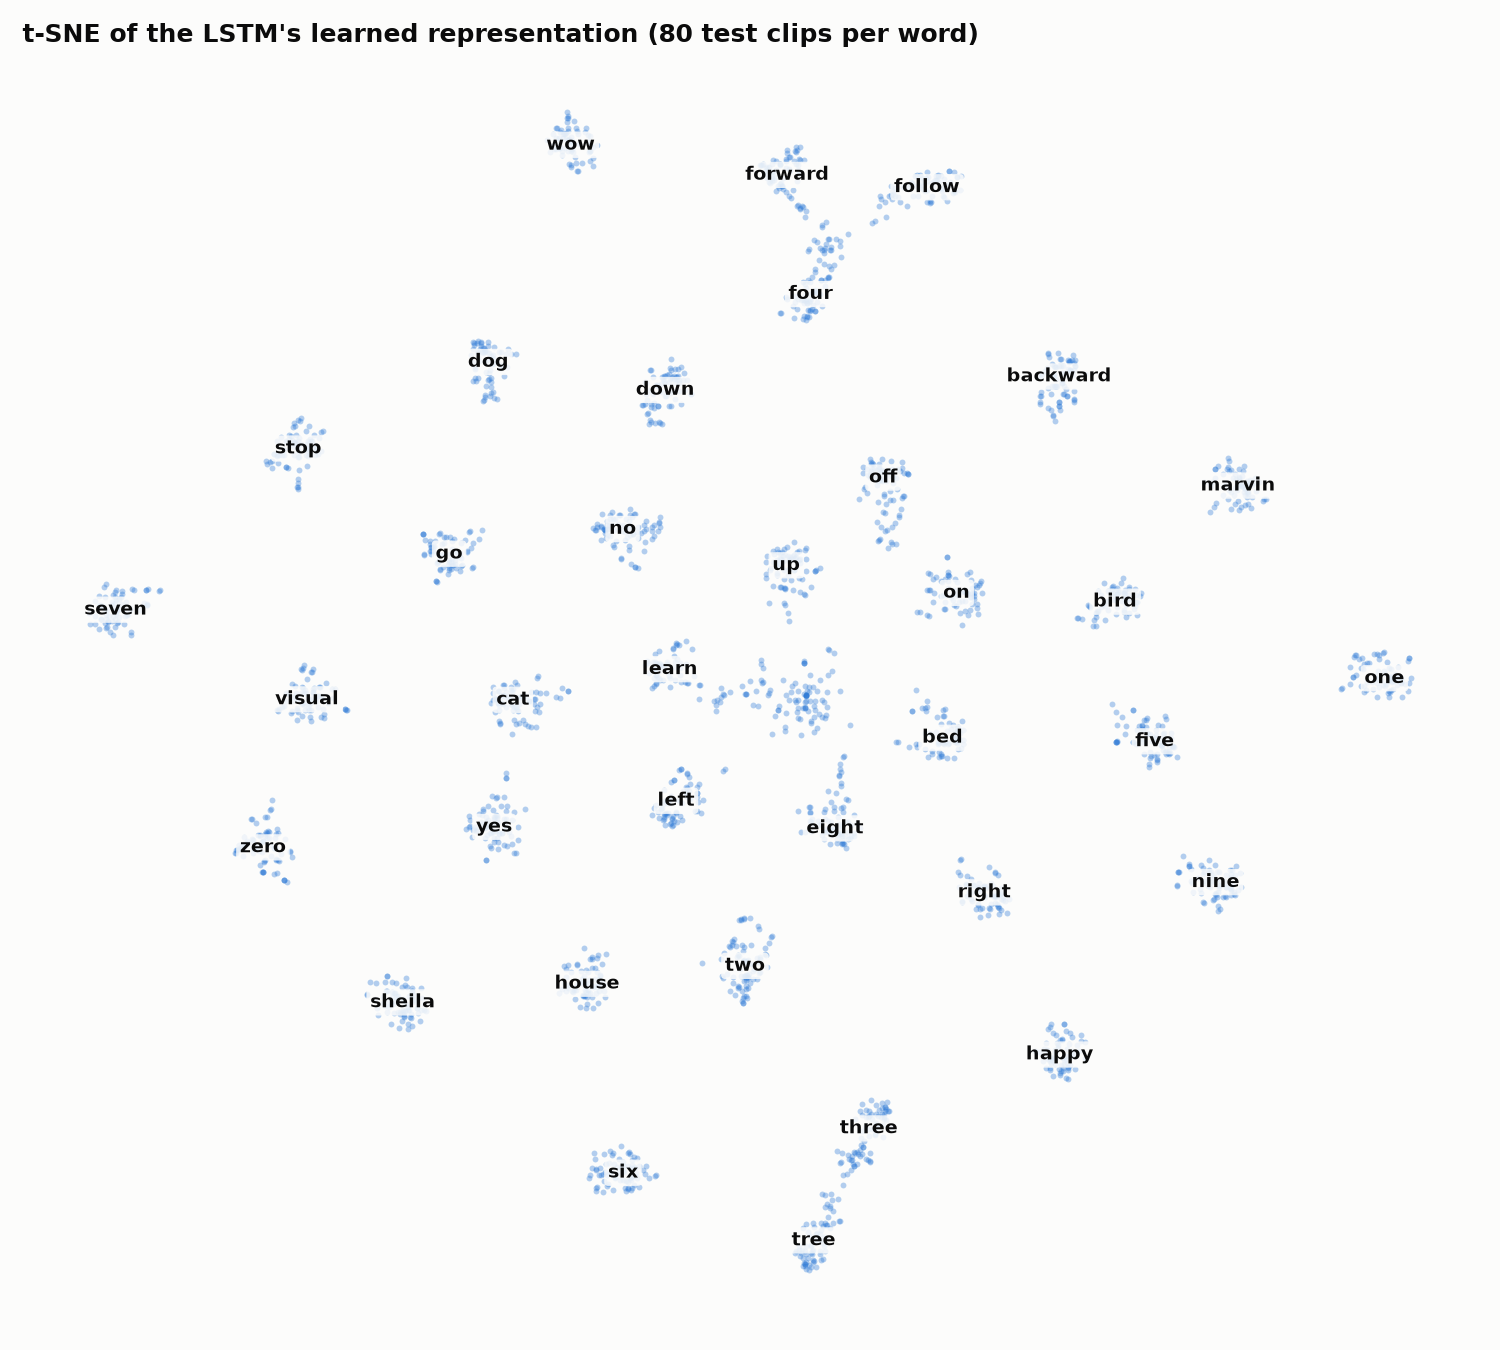
\includegraphics[width=0.82\textwidth]{../outputs/report/08_embeddings_tsne.png}
\caption{Projeção t-SNE da camada oculta de $512$ dimensões para $80$ clipes de teste de cada palavra. O rótulo de cada grupo está na posição média dos seus pontos.}
\label{fig:tsne}
\end{figure}

Na Figura~\ref{fig:tsne} cada palavra forma um grupo próprio e compacto. As palavras que se tocam são as mesmas que a matriz de confusão aponta: \w{three} e \w{tree} estão ligadas por uma ponte de pontos na parte de baixo, \w{four}, \w{forward} e \w{follow} formam um grupo de três braços no alto, e \w{off}, \w{up} e \w{on} ficam lado a lado no centro. Perto do centro há também uma nuvem difusa de pontos que não pertencem com clareza a nenhum grupo e que fica próxima de \w{learn} e \w{left}; são provavelmente clipes difíceis ou mal rotulados. As palavras sem vizinho parecido, como \w{seven}, \w{one}, \w{wow} e \w{sheila}, ficam isoladas na borda. Como em qualquer t-SNE, só a vizinhança tem significado; o tamanho dos grupos e a distância entre grupos afastados não podem ser lidos como medidas.

\section{Conclusão}

Tratando cada clipe como uma série temporal de $101$ espectros log-mel, uma LSTM bidirecional de duas camadas classificou as $35$ palavras do Speech Commands v0.02 com $95{,}1\%$ de acurácia em locutores que não estavam no treino, contra $2{,}9\%$ do acaso. Os resultados vêm de uma divisão por locutor verificada, de estatísticas de normalização e aumento de dados restritos ao treino e de um teste avaliado uma só vez. O aumento de dados explica a validação acima do treino e deu ao modelo tolerância a ruído conhecido: a acurácia fica acima de $87\%$ até $10\,\mathrm{dB}$ de SNR. Os erros que restam são pares de palavras quase iguais, como \w{tree}/\w{three}, \w{four}/\w{forward}, \w{off}/\w{up} e \w{learn}/\w{left}, e uma parte dos erros mais confiantes parece vir de rótulos errados no próprio conjunto. A suavização de rótulos deixou o modelo subconfiante (ECE de $0{,}085$). Faltaria testar a robustez com ruídos que a rede não viu no treino.

\begin{thebibliography}{9}
\bibitem{warden2018} P.~Warden. \textit{Speech Commands: A Dataset for Limited-Vocabulary Speech Recognition}. arXiv:1804.03209, 2018. \url{https://arxiv.org/abs/1804.03209}
\bibitem{davis1980} S.~Davis e P.~Mermelstein. Comparison of parametric representations for monosyllabic word recognition in continuously spoken sentences. \textit{IEEE Transactions on Acoustics, Speech, and Signal Processing}, 28(4):357--366, 1980.
\bibitem{hochreiter1997} S.~Hochreiter e J.~Schmidhuber. Long short-term memory. \textit{Neural Computation}, 9(8):1735--1780, 1997.
\bibitem{park2019} D.~S.~Park, W.~Chan, Y.~Zhang, C.-C.~Chiu, B.~Zoph, E.~D.~Cubuk e Q.~V.~Le. SpecAugment: A Simple Data Augmentation Method for Automatic Speech Recognition. \textit{Interspeech}, 2019. arXiv:1904.08779.
\end{thebibliography}

\end{document}
